\documentclass[10pt]{article}
\usepackage{mathtools}
\usepackage{fancybox}
\usepackage{tikz}
\usepackage[margin=1.5in]{geometry}
\DeclarePairedDelimiter{\ceil}{\lceil}{\rceil}
\DeclarePairedDelimiter\floor{\lfloor}{\rfloor}

\begin{document}
\vspace*{\fill}
\begin{Huge}
\begin{center}
HW1\\
Name: Ayush Jain\\
UNI: aj2672
\end{center}
\end{Huge}
\vspace*{\fill}
\newpage
Problem 1.1\\
$(an+b)^d = \theta(n^d)$ \\
$(an + b)^d = n^d(a + b/n)^d.$
As n grows and reaches infinity, the above equation tends to $(an)^d$. 
Hence, it is true to say, 
$(an+b)^d = \theta(n^d)$ 
\\\\\\\\
Problem 1.2\\
Lets assume, $3^{4n} = O(2^{4n})$\\
Which means there exists positive values c and $n_{o}$ so that, $$3^{4n} \leq c2^{4n}$$ for all $n > n_{o}$.\\
i.e. $4n log3 \leq logc + 4n log2$\\
$4nlog3 \leq logc + 4n$\\
$4n(log3/2) \leq logc$\\
There do not exists any possible values of c and $n_{o}$ for which the above holds true. Hence, $3^{4n} \neq O(2^{4n})$\\
\\
\\
\\

$3^{4n} = 2^{O(4n)}$\\
i.e $4nlog3 = O(4n)log2$\\
$4nlog3/log2 = O(4n)$\\
$4nlog3/log2 \leq c4n$ for all $n > n_{o}$\\
On comparing, we get $n_{o} = 0$ and for all $c > log3/log2$, the above holds true.\\
Hence, $3^{4n} = 2^{O(4n)}$\\



\newpage
\setcounter{equation}{0}
Problem 2.
For a function to be polynomially bounded, \\
$f(n) \leq cn^k$\\
$\log (f(n)) \leq k\log n\\
\log (f(n)) = O(\log n)$\\\\
Assuming that $f(n) = \ceil{\log n}!$ is polynomially bounded : \\
$ \log (\log n)! \leq \log \ceil {\log n}! \leq c\log n $
\\Let $\log n = k$\\
Then, $\log k! \leq ck$\\
$\theta(k\log k) \neq O(k)$
\\Hence, our assumption was wrong and $f(n) = \ceil{\log n}!$ is not polynomially bounded.
\\\\
Again, doing the same for $f(n) = \ceil{\log \log n}!$\\
$ \log (\log \log n)! \leq \log \ceil {\log \log n}! \leq c\log n $
\\Let, $\log \log n = k$\\
Then, $\log k! \leq c2^k$\\
$\theta(k\log k) \leq O(2^k)$ which is true. 
\\Hence, our assumption was right and $f(n) = \ceil{\log \log n}!$ is polynomially bounded.

\newpage
\setcounter{equation}{0}
Problem 3.

3-4 a. $f(n) = O(g(n))$ implies $g(n) = O(f(n))$\\
\begin{center}
f(n) = O(g(n))
\end{center}
$f(n) \leq cg(n)$
for all $n > n_{o}$\\
Which does not necessarily prove that g(n) = O(f(n))

For example, we know that
\begin{center}
$2^n = O(3^n)$
\end{center}
However, \begin{center} $3^n \neq O(2^n)$ \end{center}
Hence the statement is false.\\\\\\\\\\\\
3-4 b. $f(n) + g(n) = \theta(min(f(n), g(n)))$\\
When, f(n) and g(n) are both asymptotically positive functions. We can say that, \\
$f(n) + g(n) \leq f(n) $ and $f(n) + g(n) \leq g(n)$\\
Or, $f(n) + g(n) \leq min(f(n), g(n))$\\
Hence, 
\begin{center}
f(n) + g(n) = O(min(f(n), g(n))
\end{center}
However, $f(n) + g(n) \geq min(f(n), g(n))$ is not always true.\\
Hence, $f(n) + g(n) \neq \theta(min(f(n), g(n))$
\\\\\\\\\\\
3-4 g. $f(n) = \theta(f(n/2))$\\
$f(n) = \theta(f(n/2))$ is true, if $f(n) = O(f(n/2))$ and $f(n) = \Omega(f(n/2))$ is true\\
Lets take, $f(n) = 2^n$\\
if, $f(n) = O(f(n/2))$\\
it means there exists positive constants c and $n_{o}$ such that,\\
$2^n \leq c2^{n/2}$ for all $n>n_{o}$\\
i.e. $2^{n/2} \leq c$\\
\begin{equation}
(n/2)log2 \leq logc
\end{equation}
There does not exist any combination of c and $n_{o}$, so that (1) is true. Hence $f(n) \neq O(f(n/2))$
Hence, $f(n) = \theta(f(n/2))$ is false.\\\\\\\\\\\
3-4 h. $f(n) + o(f(n) = \theta(f(n)$\\
\setcounter{equation}{0}
Lets define a function g(n) such that, $g(n) = o(f(n)$
Which means, there exists positive constants c and $n_{o}$ such that,\\
$g(n) \leq cf(n)$ for all $n \geq n_{o}$
Adding f(n) to both sides, we can also say: \\
$f(n) + g(n) \leq (c+1)f(n)$\\
i.e. $f(n) + g(n) \leq Cf(n)$
\begin{equation}
f(n) + o(f(n) = O(f(n))
\end{equation}
Also, since $g(n) \geq 0$,
$f(n) + g(n) \geq f(n)$
Hence, 
\begin{equation}
f(n) + o(f(n)) = \Omega(f(n)
\end{equation}
From (1) and (2),
\begin{center}
$f(n) + o(f(n)) = \theta(f(n)$
\end{center}



\newpage
Problem 4\\
Increasing order of growth is:
$4^{loglogn} < (logn)^3 < (logn)^{logn/loglogn} = 16n + 10000 < n^{1.01} < n^2-n/logn = n^2 = 4^{logn} < 3^{n/2} < 2^n $\\

Now, we will prove the order by taking two adjacent functions at a time.\\\\
1. $4^{loglogn} < (logn)^3 $\\
Taking log on both sides, LHS becomes : $2loglogn$\\ 
RHS : $3loglogn$\\
$LHS < RHS$. Hence, $4^{loglogn} $ grows at a slower rate as compared to $ (logn)^3 $
\\\\
2. $(logn)^3 < (logn)^{logn/loglogn}$\\
Taking log on both sides, LHS becomes : $3loglogn$\\
RHS: $(loglogn)(logn/loglogn) = logn$\\
We know that, $logn$ grows at a faster rate as compared to $loglogn$. Hence, $(logn)^{logn/loglogn}$ grows faster than $(logn)^3$
\\\\
3. $(logn)^{logn/loglogn} = 16n + 10000$\\
Again, if we take log on both sides we get:\\
LHS : $logn$\\
RHS : $log(16n + 10000)$\\
O(log(f(n))) for both functions is logn. Hence, O(f(n) = n. Thus, both grow at the same rate.
\\\\
4. $16n+10000 < n^{1.01}$\\
Its easy to see in the above case that LHS grows as a power 1 of n while the RHS grows as a power of 1.01. Hence the growth rate of RHS will be higher.
\\\\
5. $n^{1.01} < n^2 - n/logn$\\
$n^2 - n/logn = n(n - 1/logn)$\\
At high values of n, RHS will grow as a function of $n^2$, faster as compared to $n^{1.01}$.
\\\\
6. $n^2 - n/logn = n^2$\\
For positive values of n, $n^2 - n/logn$ is always less than $n^2$. However both the functions grow at a rate of $n^2$.
\\\\
7. $n^2 = 4^{logn}$\\
Taking log on both sides :\\ 
LHS : $2logn$\\
RHS : $lognlog4 = 2logn$\\
Hence, it can be seen that the two functions have the same growth rate.
\\\\
8. $4^{logn} <  2^n$\\
Taking log on both sides:\\
LHS : $2logn$\\
RHS : $n$\\
We know that $logn < n$. Hence the above order holds good.
\\\\
9. $ 2^n < 3^{n/2}$\\
Taking log on both sides : \\
LHS : $n$
RHS : $(n/2)log 3$\\
Since, log3/2 is greater than 1, we know that $(n/2)log 3 > n$

\newpage
\setcounter{equation}{0}
Problem 5.\\
4.4-3 T(n) = 4T(n/2+2) + n\\\\
\ovalbox{
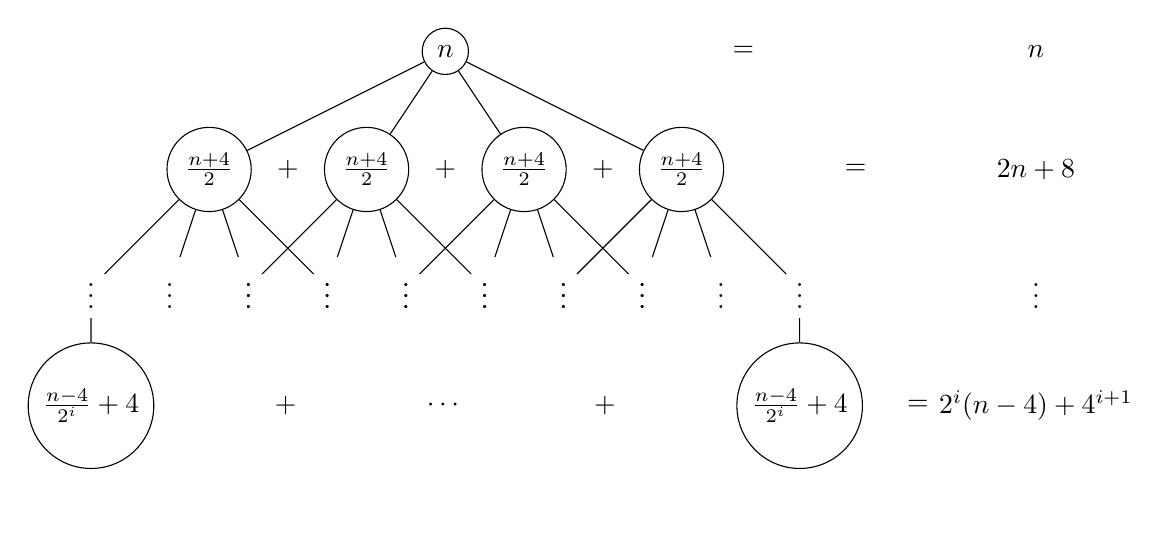
\begin{tikzpicture}[level/.style={sibling distance=20mm/#1}]
\node [circle,draw] (z){$n$}
  child {node [circle,draw] (a) {$\frac{n+4}{2}$}
  	child {node {$\vdots$}
        child {node [circle,draw] (b) {$\frac{n-4}{2^i}+4$}}
    } 
    child {node {$\vdots$}}
	child {node {$\vdots$}}
	child {node {$\vdots$}}
  }
  child {node [circle,draw] (c) {$\frac{n+4}{2}$}
  	child {node {$\vdots$}}
    child {node {$\vdots$}}
	child {node {$\vdots$}}
	child {node {$\vdots$}}
  }
  child {node [circle,draw] (d) {$\frac{n+4}{2}$}
  	child {node {$\vdots$}}
    child {node {$\vdots$}}
	child {node {$\vdots$}}
	child {node {$\vdots$}}
  }
  child {node [circle,draw] (e) {$\frac{n+4}{2}$}      
  	child {node {$\vdots$}}
    child {node {$\vdots$}}
	child {node {$\vdots$}}
	child {node {$\vdots$}
		child {node [circle,draw] (f) {$\frac{n-4}{2^i}+4$} 
  child [grow=right] {node (q) {$=$} edge from parent[draw=none]
          child [grow=right] {node (q) {$ 2^i(n-4) + 4^{i+1} $} edge from parent[draw=none]
            child [grow=up] {node (r) {$\vdots$} edge from parent[draw=none]
          	  child [grow=up] {node (t) {$2n+8$} edge from parent[draw=none]
                  child [grow=up] {node (u) {$n$} edge from parent[draw=none]}
                }
              }
            }
          }
          }
          }
          };
\path (a) -- (c) node [midway] {+};
\path (c) -- (d) node [midway] {+};
\path (d) -- (e) node [midway] {+};
\path (b) -- (f) node (x) [midway] {$\cdots$}
  child [grow=down] {
    edge from parent[draw=none]
  };
\path (b) -- (x) node [midway] {+};
\path (x) -- (f) node [midway] {+};
\path (z) -- (u) node [midway] {=};
\path (e) -- (t) node [midway] {=};
\end{tikzpicture}}\\\\
The problem size reduces to approximately 1/2 at each downward level. Hence, number of levels = $\log n$\\
T(n) at zero level = n\\
T(n) at first level = $\dfrac{4(n+4)}{2}$\\
T(n) at second level = $\dfrac{16(n+4+8)}{4}$\\
T(n) at third level = $\dfrac{64(n+4+8+16)}{8}$\\
T(n) at ith$(i > 0)$ level = $\dfrac{4^i(n+\sum_{k=1}^{i}{2^{k+1}})}{2^i}\\
 = 2^i(n+(2^2 + 2^3 + 2^4 + ..... + n))\\
 = 2^i(n + 4(2^i - 1)\\ = 2^i(n-4) + 4^{i+1}$\\
$T(n) = n$[T(n) at 0 level] + $\sum_{i=1}^{\log n}(2^i(n-4) + 4^{i+1})\\$
\begin{equation}
T(n) = n + (n-4)\sum_{i=1}^{\log n}2^i + \sum_{i=1}^{\log n}4^{i+1}\\
\end{equation}
$\sum_{i=1}^{\log n}2^i = 2 + 4 + 8 + ..... + n
 = 2n\\
\sum_{i=1}^{\log n}4^{i+1} = 4^2 + 4^3 + ...... 4n^2
 = 4n^2(1 + 1/4 + 1/16 + ....) = 16n^2/3$
\\\\Substituting into (1) : \\
$T(n) = n + (n-4)2n + 16n^2/3 = \theta(n^2) $
\\\\
Verification: We prove for $T(n) = O(cn^2 - dn)$ which will automatically imply that $T(n) = O(cn^2)\\
T(n) = 4T(n/2+2) + n\\
T(n) = 4c(n/2 + 2)^2 - d(n/2+2) + n\\
T(n) = cn^2 + 16c + 8cn + n -2dn - 8d = O(cn^2 - dn)\\
cn^2 +16c + 8cn + n - 2dn - 8d \leq cn^2 - dn\\
16c + 8cn + n - dn - 8d \leq 0\\
n(8c + 1 -d) + 16c - 8d \leq 0$\\
The above equation holds good for c = 1/8 and d = 2.
\\\\\\\\\\\\\\\
4.4-8 T(n) = T(n-a) + T(a) + cn\\
\ovalbox{
\begin{tikzpicture}[level/.style={sibling distance=60mm/#1}]
\node [circle,draw] (z){$n$}
  child {node [circle,draw] (a) {$n-a$}
    child {node [circle,draw] (b) {$n-2a$}
      child {node {$\vdots$}
        child {node [circle,draw] (d) {$n-ia$}}
        child {node [circle,draw] (e) {$a$}}
      } 
      child {node [circle,draw] (f) {$a$}}
    }
    child {node [circle,draw] (g) {$a$}
    }
  }
  child {node [circle,draw] (j) {$a$}
    }   child [grow=right] {node (q) {$=$} edge from parent[draw=none]
          child [grow=right] {node (q) {$ cn $} edge from parent[draw=none]
            child [grow=down] {node (r) {$c(n-a) + T(a)$} edge from parent[draw=none]
              child [grow=down] {node (s) {$c(n-2a) + T(a)$} edge from parent[draw=none]
                child [grow=down] {node (t) {$\vdots$} edge from parent[draw=none]
                  child [grow=down] {node (u) {$c(n-ia) + T(a)$} edge from parent[draw=none]}
                }
              }
            }
          }
        };
\path (q) -- (r) node [midway] {+};
\path (s) -- (r) node [midway] {+};
\path (s) -- (t) node [midway] {+};
\path (r) -- (j) node [midway] {=};
\path (t) -- (u) node [midway] {+};
\path (e) -- (u) node [midway] {=};
\path (j) -- (t) node [midway] {=};
\end{tikzpicture}}\\\\
So, at each level the problem size decreases by a. The tree expands till $n-ia \leq a => i = n/a-1$\\
At each level, work = T(a) + c(n-ia).\\
Total work = $\sum_{i=0}^{n/a-1}(T(a) + c(n-ia))\\
= T(a)n/a + cn(n/a) - ca(n/a)(n/a-1)/2\\
= cn^2/2a + n(T(a)-1)\\\
= \theta(n^2)$\\
\\\\\\\\
4-3 b. $T(n) = 3T(n/3) + n/\log n$\\
Let $\log n = k\\
T(3^k) = 3T(3^{k-1}) + 3^k/k\\
T(3^k)/3^k = T(3^{k-1})/3^{k-1} + 1/k$\\
Let, $T(3^k)/3^k = S(k)$\\
S(k) = S(k-1) + 1/k\\\\
\ovalbox{
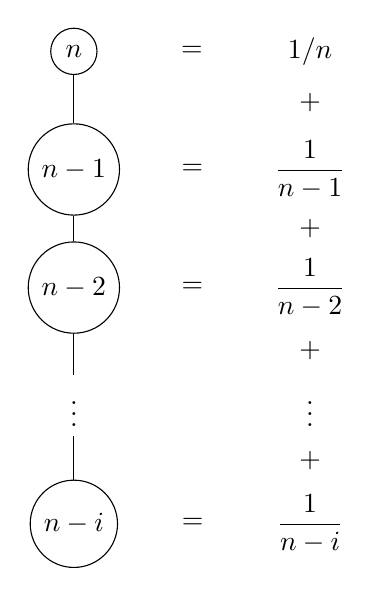
\begin{tikzpicture}[level/.style={sibling distance=0mm/#1}]
\node [circle,draw] (z){$n$}
  child {node [circle,draw] (a) {$n-1$}
    child {node [circle,draw] (b) {$n-2$}
      child {node {$\vdots$}
        child {node [circle,draw] (d) {$n-i$}}
      } 
    }
  }
    child [grow=right] {node (q) {$=$} edge from parent[draw=none]
          child [grow=right] {node (q) {$ 1/n $} edge from parent[draw=none]
            child [grow=down] {node (r) {$\dfrac{1}{n-1}$} edge from parent[draw=none]
              child [grow=down] {node (s) {$\dfrac{1}{n-2}$} edge from parent[draw=none]
                child [grow=down] {node (t) {$\vdots$} edge from parent[draw=none]
                  child [grow=down] {node (u) {$\dfrac{1}{n-i}$} edge from parent[draw=none]}
                }
              }
            }
          }
        };
\path (q) -- (r) node [midway] {+};
\path (s) -- (r) node [midway] {+};
\path (s) -- (t) node [midway] {+};
\path (a) -- (r) node [midway] {=};
\path (t) -- (u) node [midway] {+};
\path (b) -- (s) node [midway] {=};
\path (d) -- (u) node [midway] {=};
\end{tikzpicture}}\\\\
number of level $= k$\\
Time for work done at zero level = $1/k$\\
Time for work done at first level = $1/(k-1)$\\
Time for work done at second level = $1/(k-2)$\\
Time for work done at $i^th$ level = $1/(k-i)$\\
$S(k) = 1/k + 1/(k-1) + .... 1\\
S(k) = \theta(ln k)\\
T(n)/n = \theta(\log \log n)\\
T(n) = \theta(n \log \log n)$
\\\\\\\\\\\
4-3 c. $T(n) = 4T(n/2) + n^{5/2}$\\
For the above function, $f(n) = n^{5/2}$\\
$n^{log_b a} = n^{log_2 4} = n^2$\\
Since $f(n) = \Omega(n^2) = \Omega(n^{log_b a})$\\
By master's theorem, $T(n) = \theta(n^{5/2})$
\newpage
4-3 h. T(n) = T(n-1) + logn\\\\
\ovalbox{
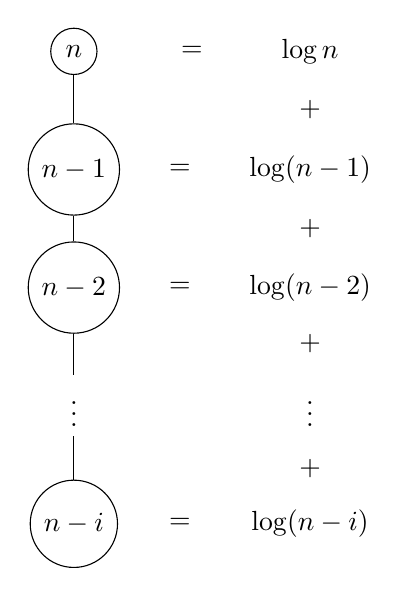
\begin{tikzpicture}[level/.style={sibling distance=0mm/#1}]
\node [circle,draw] (z){$n$}
  child {node [circle,draw] (a) {$n-1$}
    child {node [circle,draw] (b) {$n-2$}
      child {node {$\vdots$}
        child {node [circle,draw] (d) {$n-i$}}
      } 
    }
  }
    child [grow=right] {node (q) {$=$} edge from parent[draw=none]
          child [grow=right] {node (q) {$\log n $} edge from parent[draw=none]
            child [grow=down] {node (r) {$\log (n-1)$} edge from parent[draw=none]
              child [grow=down] {node (s) {$\log (n-2)$} edge from parent[draw=none]
                child [grow=down] {node (t) {$\vdots$} edge from parent[draw=none]
                  child [grow=down] {node (u) {$\log (n-i)$} edge from parent[draw=none]}
                }
              }
            }
          }
        };
\path (q) -- (r) node [midway] {+};
\path (s) -- (r) node [midway] {+};
\path (s) -- (t) node [midway] {+};
\path (a) -- (r) node [midway] {=};
\path (t) -- (u) node [midway] {+};
\path (b) -- (s) node [midway] {=};
\path (d) -- (u) node [midway] {=};
\end{tikzpicture}}\\\\
Since at each level problem size reduces by 1, no of levels = n\\
Time for work done at zero level = logn\\
Time for work done at first level = log(n-1)\\
Time for work done at second level = log(n-2)\\
Time for work done at ith level = log(n-i)\\
T(n) = $\sum_{i=0}^{n-1} log(n-i)\\
 = (\log n + \log (n-1) + \log (n-2) + .... + log (n-n+1)\\
 = \log n(n-1)(n-2)...1 \\
 = \theta(\log n!) = \theta(nlogn)$
\\\\\\\\\\\\ 
4-3 j. $T(n) = \sqrt{n}T(\sqrt{n}) + n$\\
Dividing by n :
$T(n)/n = T(\sqrt{n})/\sqrt{n} + 1$\\
Let T(n)/n = S(n)\\
Then, $S(n) = S(\sqrt{n}) + 1$\\
Let $n = 2^k\\
S(2^k) = S(2^{k/2}) + 1$\\
Renaming, $R(k) = S(2^k)$\\
$R(k) = R(k/2) + 1$\\\\
\ovalbox{
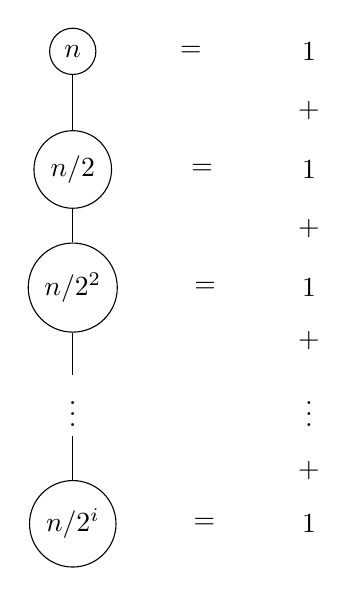
\begin{tikzpicture}[level/.style={sibling distance=0mm/#1}]
\node [circle,draw] (z){$n$}
  child {node [circle,draw] (a) {$n/2$}
    child {node [circle,draw] (b) {$n/2^2$}
      child {node {$\vdots$}
        child {node [circle,draw] (d) {$n/2^i$}}
      } 
    }
  }
    child [grow=right] {node (q) {$=$} edge from parent[draw=none]
          child [grow=right] {node (q) {$1$} edge from parent[draw=none]
            child [grow=down] {node (r) {$1$} edge from parent[draw=none]
              child [grow=down] {node (s) {$1$} edge from parent[draw=none]
                child [grow=down] {node (t) {$\vdots$} edge from parent[draw=none]
                  child [grow=down] {node (u) {$1$} edge from parent[draw=none]}
                }
              }
            }
          }
        };
\path (q) -- (r) node [midway] {+};
\path (s) -- (r) node [midway] {+};
\path (s) -- (t) node [midway] {+};
\path (a) -- (r) node [midway] {=};
\path (t) -- (u) node [midway] {+};
\path (b) -- (s) node [midway] {=};
\path (d) -- (u) node [midway] {=};
\end{tikzpicture}}\\\\

No of level for this recurrence tree = $\log n$\\
R(k) = $(1+1+1+ ..... + \log k times)$\\
 $= \log k$\\
R(k) = $\log k$\\
$R(k) = S(2^k) = S(n) = T(n)/n = \log \log n$\\
T(n) = $n(\log \log n)$\\

\newpage
\setcounter{equation}{0}
Problem 4-5. Chip testing.\\
a. We know that bad chips cannot be trusted with their decision because they can go in any direction. To reach a certain conclusion we need to be sure that majority of observations coming through pairwise testing are correct, otherwise the test fails.\\
Lets take an example of 4 chips. If 2 chips are good and 2 chips are bad, on pairwise testing we will get two cases:\\
Case 1: One group has both good chips while the other group has both bad chips. So, all the four results can say that the other chip is good and the test will fail.\\
Case 2: Both the groups have 1 good chip and 1 bad chip. In this case as well, the results from both the groups can be same and there will not be any way to know for sure.\\
However, if there were 3 good chips and 1 bad chip. One group will point out that both chips are good while the other group will say that at least one of thee chip is bad. And we will know for sure that we can take a good chip from the first group.

b. To determine a single good chip, we can follow the following algorithm based on the results. Lets G denotes the case when chip A says B is good and the B denotes the result where A says B is bad.\\
So, on pairwise testing:\\
1) if the result is (G,G), we discard one of the chips
2) if the result is (G,B) or (B,B) we discard both.
3) if the total number of chips is odd, we keep the chip left alone.
In this case, since we are discarding at least one chip from each pair, we are left with at most $ceil{n/2}$ chips at the end of one level of pairwise test.\\
This works because for all combinations of chips. Lets assume we have n chips out of which $\floor*{n/2+1}$ chips are good. Now, n can be even or odd.
Case I: n is even, out of which n/2+1 chips are good while n/2-1 chips are bad. Since the number of good chips are 2 more than the number of bad chips, we will have atleast one group of both good chips. The other groups can either be formed of one good chip and one bad chip each or they can be both good or both bad. So, after first level testing, we will be left with at one good chip from the pair of both good chips while the discarded chips will have bad chips less than or equal to the disarded good chips. Hence, the majority of the good chips will be maintained.\\
Case II: n is odd. Out of which n+1/2 are good and n-1/2 are bad. In this case we will have a left alone chip. If the left alone chip is good, the combined distribution of groups will have equal number of good and bad chips. In this case, the left alone good chip will be carried forward, while the rest of the chips will have atleast equal number of good and bad chip distribution. If the left alone chip was bad, then in the groups formed, there will be at least one group of both good chips and hence, once again the majority will be maintained.
These pairwise tests performed continuously will leave us with one good chip in the end.

c. If we have one good chip, we can test all the other chips with that good chip and trust the result it gives to find the other good chips.\\
The recurrence tree will be represented by the order:\\
\begin{equation}
T(n) = T(n-1) + 1 
\end{equation}
\\Since each test reduces the problem size by 1 and takes 1 unit of time.\\
The recurrence tree can be drawn as:\\\\
\ovalbox{
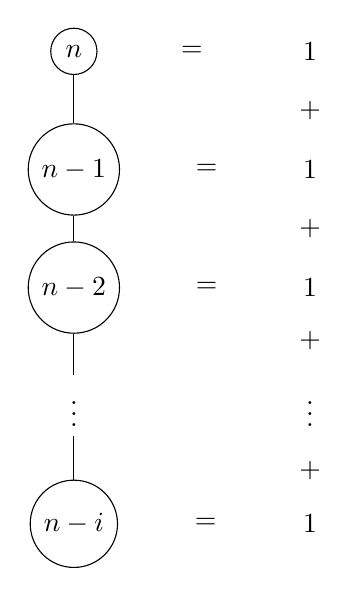
\begin{tikzpicture}[level/.style={sibling distance=0mm/#1}]
\node [circle,draw] (z){$n$}
  child {node [circle,draw] (a) {$n-1$}
    child {node [circle,draw] (b) {$n-2$}
      child {node {$\vdots$}
        child {node [circle,draw] (d) {$n-i$}}
      } 
    }
  }
    child [grow=right] {node (q) {$=$} edge from parent[draw=none]
          child [grow=right] {node (q) {$1$} edge from parent[draw=none]
            child [grow=down] {node (r) {$1$} edge from parent[draw=none]
              child [grow=down] {node (s) {$1$} edge from parent[draw=none]
                child [grow=down] {node (t) {$\vdots$} edge from parent[draw=none]
                  child [grow=down] {node (u) {$1$} edge from parent[draw=none]}
                }
              }
            }
          }
        };
\path (q) -- (r) node [midway] {+};
\path (s) -- (r) node [midway] {+};
\path (s) -- (t) node [midway] {+};
\path (a) -- (r) node [midway] {=};
\path (t) -- (u) node [midway] {+};
\path (b) -- (s) node [midway] {=};
\path (d) -- (u) node [midway] {=};
\end{tikzpicture}}\\\\
Hence, T(n) = 1+ 1+1+ .... + n-1 times\\
$T(n) = \theta(n)$

\newpage
\begin{huge}
\begin{center}
References
\end{center}
\end{huge}
1) Discussed question 4.4-3 and 4-3 b with Prateek Gupta
\end{document}